% !TEX root = ../master/master.tex

%% Dexter Barrows, 2016
%% dbarrows.github.io


	Markov Chain Monte Carlo (MCMC) is a general class of methods designed to sample from the posterior distribution of model parameters \cite{Andrieu2003}. It is an algorithm used when we wish to fit a model $M$ that depends on some parameter (or more typically vector of parameters) $\theta$ to observed data $D$. MCMC works by constructing a Markov chain whose stationary distribution converges to desired posterior distribution. The samples drawn using MCMC are used to numerically approximate the stationary distribution, and in turn the posterior \cite{Andrieu2003}.


\section{Markov Chains}

    Figure [\ref{fsm}] shows a finite state machine with 3 states $S = \{x_1, x_2, x_3\}$.

    \begin{figure}
        \centering
        \captionsetup{width=0.8\linewidth}
        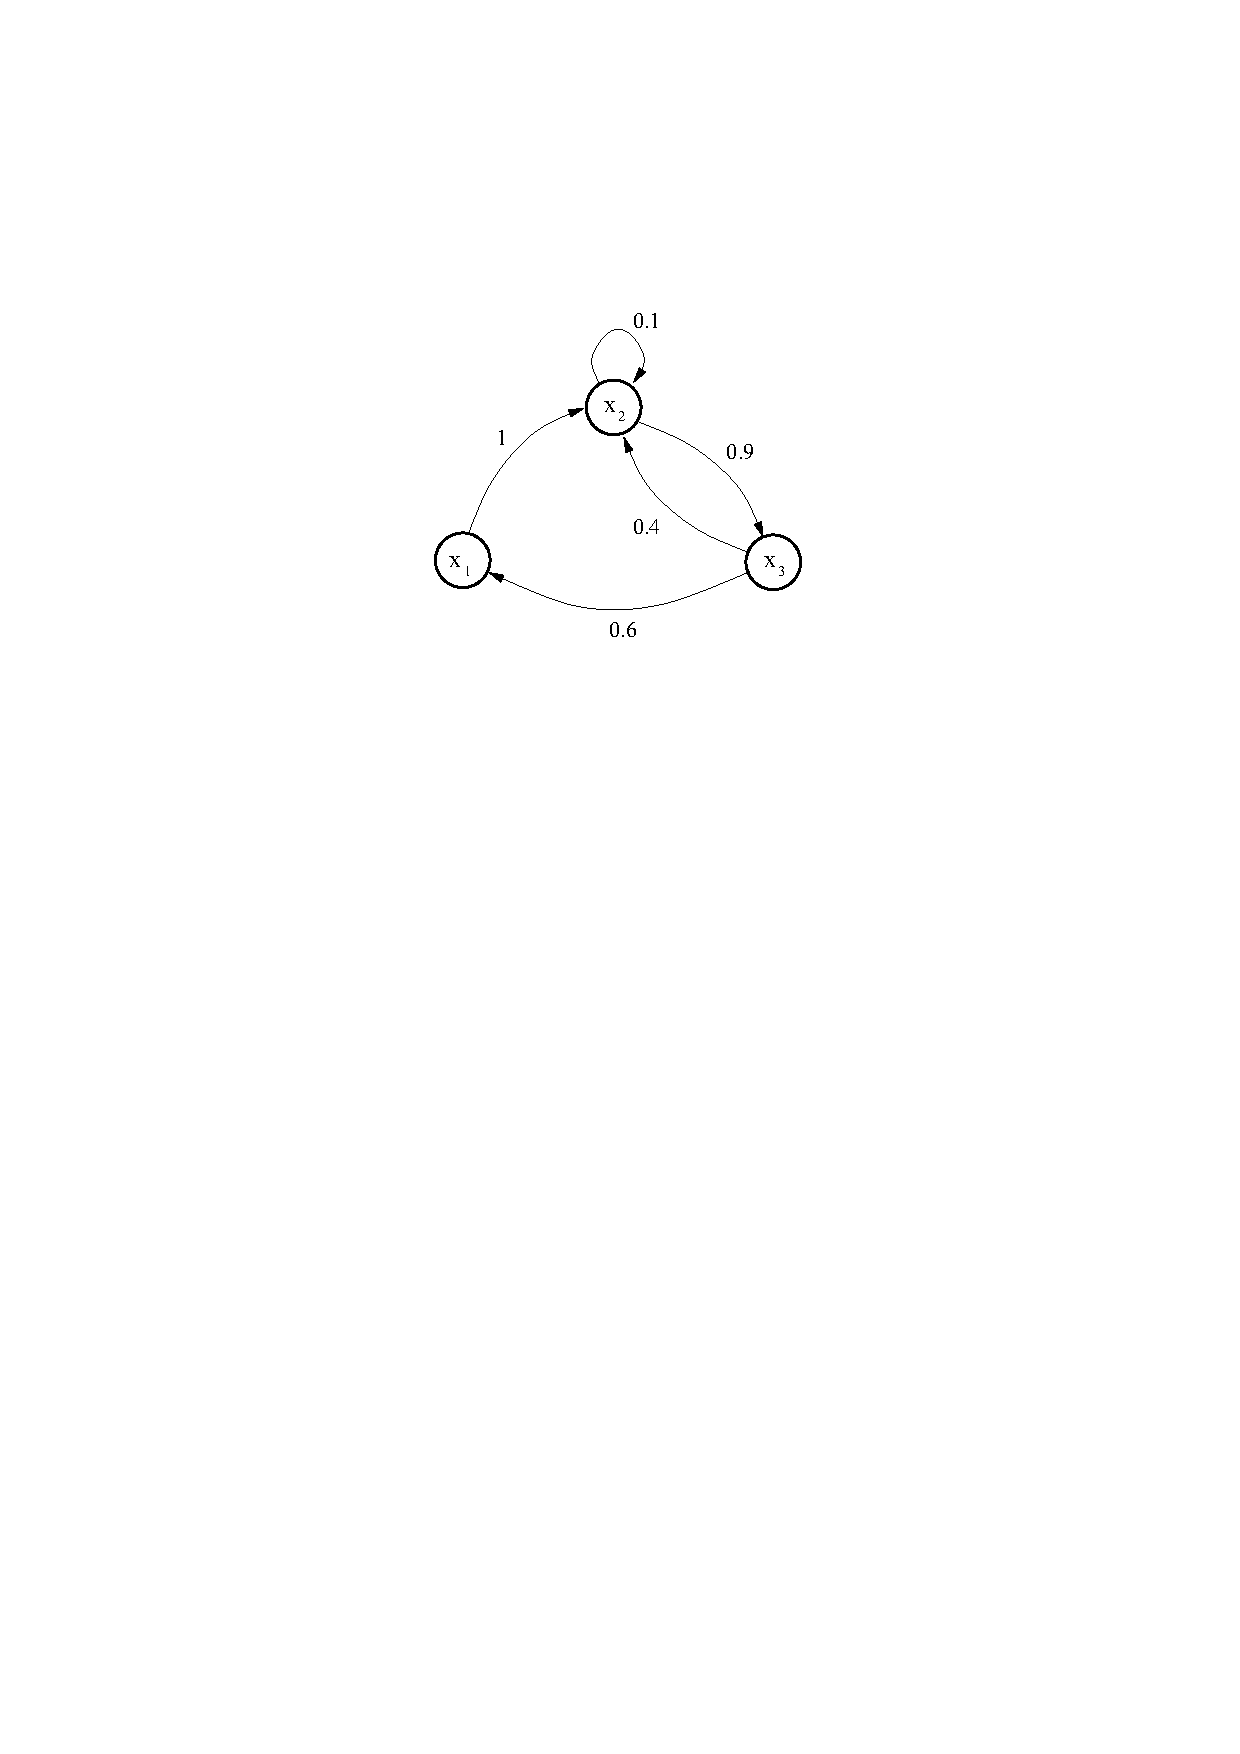
\includegraphics[width=0.5\textwidth]{./images/finitemachine.pdf}
        \caption{A finite state machine. States are shown as graph nodes, and the probability of transitioning from one particular state to another is shown as a weighted graph edge. \cite{Andrieu2003} \label{fsm}}
    \end{figure}

    The transition probabilities can be summarized as a matrix as

    \begin{equation}
    	T = 
	    \begin{bmatrix}
	        0 & 1 & 0 \\
	        0 & 0.1 & 0.9 \\
	        0.6 & 0.4 & 0
	    \end{bmatrix}.
    \end{equation}

    The probability vector $\mu(x^{(1)})$ for a state $x^{(1)}$ can be evolved using $T$ by evaluating $\mu(x^{(1)})T$, then again by evaluating $\mu(x^{(1)})T^2$, and so on. If we take the limit as the number of transitions approaches infinity, we find

    \begin{equation}
    	\lim_{t \to \infty} \mu(x^{(1)})T^t = (27/122, 50/122, 45/122).
    \end{equation}

    This indicates that no matter what we pick for the initial probability distribution $\mu(x^{(1)})$, the chain will always stabilize at the equilibrium distribution.

    This property holds when the chain satisfies the following conditions

    \begin{itemize}
        \item \textit{Irreducible} Any state A can be reached from any other state B with non-zero probability
        \item \textit{Positive Recurrent} The number of steps required for the chain to reach state A from state B must be finite
        \item \textit{Aperiodic} The chain must be able to explore the parameter space without becoming trapped in a cycle
    \end{itemize}

    Note that MCMC sampling generates a Markov chain $(\theta^{(1)}, \theta^{(2)},..., \theta^{(N)})$ that does indeed satisfy these conditions, and uses the chain's equilibrium distribution to approximate the posterior distribution of the parameter space \cite{Andrieu2003}.    


\section{Likelihood}

    MCMC and similar methods hinge on the idea that the weight or support bestowed upon a particular set of parameters $\theta$ should be proportional to the probability of observing the data $D$ given the model output using that set of parameters $M(\theta)$. In order to do this we need a way to evaluate whether or not $M(\theta)$ is a good fit for $D$; this is done by specifying a likelihood function $\mathcal{L}(\theta)$ such that

    \begin{equation}
    	\mathcal{L}(\theta) \propto P(D|\theta).
    \end{equation}

    In frequentist Maximum Likelihood approaches, $\mathcal{L}(\theta)$ is searched to find a value of $\theta$ that maximizes $\mathcal{L}(\theta)$, then this $\theta$ is taken to be the most likely true value. Bayesian approaches take this further by aiming to generate a posterior distribution of likelihood values conditioned on prior information about the parameters and the data -- to not just maximize the likelihood but to also explore the area around it \cite{Andrieu2003}.


\section{Prior distribution}

    Another significant component of MCMC is the user-specified prior distribution for $\theta$ or distributions for the individual components of $\theta$ (priors). Priors serve as a way for us to tell the MCMC algorithm what we think consist of good values for the parameters. Note that if very little is known about the parameters, or we are worried about biasing our estimate of the posterior, we can simply use a a wide uniform distribution. We cannot, however, avoid this problem entirely. Bayesian frameworks, such as MCMC, \textit{require} priors to be specified; what the user must decide is how strong to make priors.

   	Exceedingly weak priors can prove problematic in some circumstances. In the case of MCMC, weak priors handicap the algorithm in two ways: convergence of the chain may become exceedingly slow, and more pressure is put on the likelihood function to be as good as possible -- it will now be the only thing informing the algorithm of what constitutes a ``good'' set of parameters, and what should be considered poor. In the majority of cases this does not pose as much as a problem as it would appear; if enough samples are drawn, we should still obtain a good posterior estimate. We will only really run into problems if an exceedingly weak prior, such as an unbounded uniform distribution, or another unbounded distribution with a high standard deviation, is specified -- in those cases we may obtain poor posterior estimates if the data are weak \cite{Andrieu2003}.

\section{Proposal distribution}

    As part of the MCMC algorithm, when we find a state in the parameter space that is accepted as part of the Markov chain construction process, we need a good way of generating a good next step to try. Unlike basic rejection sampling in which we would just randomly sample from our prior distribution, MCMC attempts to optimise our choices by choosing a step that is close enough to the last accepted step so as to stand a decent chance of also being accepted, but far enough away that it doesn't get ``trapped'' in a particular region of the parameter space.

    This is done through the use of a proposal or candidate distribution. This will usually be a distribution centred around our last accepted step and with a dispersion potential narrower than that of our prior distribution.

    The choice of this distribution is theoretically not of the utmost importance, but in practice becomes important so as to not waste computer time \cite{Andrieu2003}.


\section{Algorithm}

    Now that we have all the pieces necessary, we can discuss the details of the MCMC algorithm.

    We will denote the previously discussed quantities as

    \begin{itemize}
        \item $p(\cdot)$ - the prior distribution
        \item $q(\cdot|\cdot)$ - the proposal distribution
        \item $\mathcal{L}(\cdot)$ - the Likelihood function
        \item $\mathcal{U}(\cdot,\cdot)$ - the uniform distribution
    \end{itemize}

    and the define the acceptance ratio, $r$, as

    \begin{equation}
    	r = \frac{\mathcal{L}(\theta^*)p(\theta^*)q(\theta^*|\theta)}{\mathcal{L}(\theta)p(\theta)q(\theta|\theta^*)},
    \end{equation}

    where $\theta^*$ is the proposed sample to draw from the posterior, and $\theta$ is the last accepted sample. This is known as the Metropolis-Hastings rule.

    In the special case of the Metropolis variation of MCMC, the proposal distribution is symmetric, meaning $q(\theta^*|\theta) = q(\theta|\theta^*)$, and so the acceptance ratio simplifies to

    \begin{equation}
    	r = \frac{\mathcal{L}(\theta^*)p(\theta^*)}{\mathcal{L}(\theta)p(\theta)}.
    \end{equation}

    Algorithm [\ref{mhmcmc}] shows the Metropolis MCMC algorithm.
    
    \begin{algorithm}

        \BlankLine

        \SetKwInOut{Input}{Input}
        \SetKwInOut{Output}{Output}
        \DontPrintSemicolon

        \tcc{Select a starting point}
        \Input{Initialize $\theta^{(1)}$}

        \BlankLine

        \For{$i = 2:N$}{

            \BlankLine

            \tcc{Sample}
            $\theta^* \sim q(\cdot|\theta^{(i-1)})$ \;
            $u \sim \mathcal{U}(0,1)$

            \BlankLine

            \tcc{Evaluate acceptance ratio}
            $r$ $\gets$ $\frac{\mathcal{L}(\theta^*)p(\theta^*)}{\mathcal{L}(\theta)p(\theta)}$

            \BlankLine

            \tcc{Step acceptance criterion}
            \eIf{ $u < \min\left\{ 1 , r \right\}$ }{ 
                $\theta^{(i)} = \theta^*$\;
            }{
                $\theta^{(i)} = \theta^{(i-1)}$\;
            }
        }

        \BlankLine

        \tcc{Samples from approximated posterior distribution}
        \Output{Chain of samples $(\theta^{(1)},\theta^{(2)},...,\theta^{(N)})$}

        \BlankLine

        \caption{Metropolis MCMC \label{mhmcmc}}

    \end{algorithm}
    

    In this way we are ensuring that steps that lead to better likelihood outcomes are likely to be accepted, but steps that do not will not be accepted as frequently. Note that these less ``advantageous'' moves will still occur but that this is by design -- it ensures that as much of the parameter space as possible will be explored but more efficiently than using pure brute force \cite{Andrieu2003}.


\section{Burn-in}

    One critical aspect of MCMC-based algorithms has yet to be discussed. The algorithm requires an initial starting point $\theta$ to be selected, but as the proposal distribution is supposed to restrict moves to an area close to the last accepted state, then the posterior distribution will be biased towards this starting point. This issue is avoided through the use of a Burn-in period.

    Burning in a chain is the act of running the MCMC algorithm normally without saving first $M$ samples. As we are seeking a chain of length $N$, the total computation will be equivalent to generating a chain of length $M+N$ \cite{Andrieu2003}.


\section{Thinning}

    Some models will require very long chains to get a good approximation of the posterior, which will consequently require a non-trivial amount of computer storage. One way to reduce the burden of storing so many samples is by thinning. This involves saving only every $n^{\text{th}}$ step, which should still give a decent approximate of the posterior (since the chain has time to explore a large portion of the parameter space), but requires less room to store \cite{Link2012}.


\section{Hamiltonian Monte Carlo}

    The Metropolis-Hastings algorithm has a primary drawback in that the parameter space may not be explored efficiently in some circumstances -- a consequence of the rudimentary proposal mechanism. Instead, smarter moves can be proposed through the use of Hamiltonian dynamics, leading to a better exploration of the target distribution and a potential decrease in overall computational complexity. This algorithm is coined Hamiltonian MCMC (HMC) \cite{Neal2011}. Prior to the advent of HMC, some work was conducted exploring adaptive step-sizing using MCMC-based methods, but found they lack strong theoretical justification, and can lead to some samples being drawn from an incorrect distribution \cite{Neal2011}. HMC has in fact existed for nearly the same amount of time as MCMC -- both methods having been developed to model molecular dynamics, with MCMC taking a probabilistic approach and HMC taking a more deterministic one -- but had not received much attention outside its native discipline until recently.

    From physics, we will borrow the ideas of potential and kinetic energy. Here potential energy is analogous to the negative log likelihood of the parameter selection given the data, formally

    \begin{equation}
        U(\theta) = -\log(\mathcal{L}(\theta)p(\theta)).
    \end{equation}

    Kinetic energy will serve as a way to ``nudge'' the parameters along a different moment for each component of $\theta$. We introduce $n$ auxiliary variables $r = (r_1, r_1,...,r_n)$, where $n$ is the number of components in $\theta$. Note that the samples drawn for $r$ are not of interest, they are only used to inform the evolution of the Hamiltonian dynamics of the system. We can now define the kinetic energy as

    \begin{equation}
        K(r) = \frac{1}{2} r^T M^{-1} r,
    \end{equation}

    where $M$ is an $n \times n$ matrix. In practice $M$ can simply be chosen as the identity matrix of size $n$, however it can also be used to account for correlation between components of $\theta$.

    The Hamiltonian of the system is defined as

    \begin{equation}
        H(\theta,r) = U(\theta) + K(r),
    \end{equation}

    where the Hamiltonian dynamics of the combined system can be simulated using the following system of ODEs:

    \begin{equation}
        \begin{array}{rl}
        \displaystyle
            \dfrac{d\theta}{dt} & = M^{-1} r \\
            \dfrac{dr}{dt} & = - \nabla U(\theta) .
        \end{array}
    \end{equation}

    It is tempting to try to integrate this system using the standard Euler evolution scheme, but in practice this leads to instability as it will not preserve the volume of the system. Instead the ``Leapfrog'' scheme is used. This scheme is very similar to Euler scheme, except instead of using a fixed step size $h$ for all evolutions, a step size of $\epsilon$ is used for most evolutions, with a half step size of $\epsilon / 2$ for evolutions of $\frac{dr}{dt}$ at the first step, and last step $L$. In this way the evolution steps ``leapfrog'' over each other while using future values from the other set of steps, leading to the scheme's name.

    The end product of the Leapfrog steps are the new proposed parameters $(\theta^*,r^*)$. These are either accepted or rejected using a mechanism similar to that of standard Metropolis-Hastings MCMC. Now, however, the acceptance ratio $r$ is defined as

    \begin{equation}\label{hmcratio}
        r = \exp \left[ H(\theta,r) - H(\theta^*,r^*) \right],
    \end{equation}

    where $(\theta,r)$ are the last values in the chain. This form of the acceptance ratio comes from the definition of the Hamiltonian as an energy function. If we define the distribution of the total potential energy in the system (known as the canonical distribution) as a function of the Hamiltonian as

    \begin{equation}
    	P(\theta,r) = \frac{1}{Z} \exp (-H(\theta,r))
    \end{equation}

    where $Z$ is a normalizing constant, then taking the ratio of the total potential energy of the proposed step $P(\theta^*,r^*)$ to the total potential energy in the last accepted step $P(\theta, r)$, we obtain Equation (\ref{hmcratio}).

    Together, we have Algorithm [\ref{hmcmc}].

    \begin{algorithm}

        \BlankLine

        \SetKwInOut{Input}{Input}
        \SetKwInOut{Output}{Output}
        \DontPrintSemicolon

        \tcc{Select a starting point}
        \Input{Initialize $\theta^{(1)}$}

        \BlankLine

        \For{$i = 2:N$}{

            \BlankLine

            \tcc{Resample moments}
            \For{$i = 1:n$}{
                r(i) $\gets$ $\mathcal{N}(0,1)$
            }

            \BlankLine

            \tcc{Leapfrog initialization}
            $\theta_0$ $\gets$ $\theta^{(i-1)}$ \;
            $r_0$ $\gets$ $r - \nabla U(\theta_0) \cdot \epsilon / 2$

            \BlankLine

            \tcc{Leapfrog intermediate steps}
            \For{$j = 1:L-1$}{
                $\theta_j$ $\gets$ $\theta_{j-1} + M^{-1} r_{j-1} \cdot \epsilon$ \;
                $r_j$ $\gets$ $r_{j-1} - \nabla U(\theta_j) \cdot \epsilon$
            }

            \BlankLine

            \tcc{Leapfrog last steps}
            $\theta^*$ $\gets$ $\theta_{L-1} + M^{-1} r_{L-1} \cdot \epsilon$ \;
            $r^*$ $\gets$ $\nabla U(\theta_L) \cdot \epsilon / 2 - r_{L-1}$            
            \BlankLine

            \tcc{Evaluate acceptance ratio}
            $r = \exp \left[ H(\theta^{(i-1)},r) - H(\theta^*,r^*) \right]$

            \BlankLine

            \tcc{Sample}
            $u \sim \mathcal{U}(0,1)$

            \BlankLine

            \tcc{Step acceptance criterion}
            \eIf{ $u < \min\left\{ 1 , r \right\}$ }{ 
                $\theta^{(i)} = \theta^*$\;
            }{
                $\theta^{(i)} = \theta^{(i-1)}$\;
            }
        }

        \BlankLine

        \tcc{Samples from approximated posterior distribution}
        \Output{Chain of samples $(\theta^{(1)},\theta^{(2)},...,\theta^{(N)})$}

        \BlankLine

        \caption{Hamiltonian MCMC \label{hmcmc}}

    \end{algorithm}

    Note that the parameters $\epsilon$ and $L$ have to be tuned in order to maintain stability and maximize efficiency, a sometimes non-trivial process utilising trial fitting with candidate values of $\epsilon$ and $L$ \cite{Neal2011}. However, some recent algorithms, such as the No U-Turn sampler implemented in RStan, and adaptively select appropriate values automatically during the sampling process \cite{Hoffman2014}.
    

\section{RStan Fitting}

    Here we will examine a test case in which Hamiltonian MCMC will be used to fit a Susceptible-Infected-Removed (SIR) epidemic model to mock infectious count data.

    The synthetic data was produced by taking the solution to a basic SIR ODE model, sampling it at regular intervals, and perturbing those values by adding in observation noise. The SIR model used was outlined in the introduction in Equation [\ref{sirode}].

    The solution to this system was obtained using the \verb|ode()| function from the \verb|deSolve| package. The required derivative array function in the format required by \verb|ode()| was specified as the gradient in Equation [\ref{sirode}].

    The true parameter values were set to $\mathcal{R}_0 = 3.0, \gamma = 0.1, N = 500$. The initial conditions were set to 5 infectious individuals, 495 people susceptible to infection, and no one had yet recovered from infection and been removed. The system was integrated over $[0,100]$ weeks with infected counts drawn at each integer time step.

    The observation error was taken to be $\varepsilon_{obs} \sim \mathcal{N}(0,\sigma)$, where individual values were drawn for each synthetic data point.

    Figure [\ref{mcmcdataplot}] shows the system simulation results.

    \begin{figure}
        \centering
        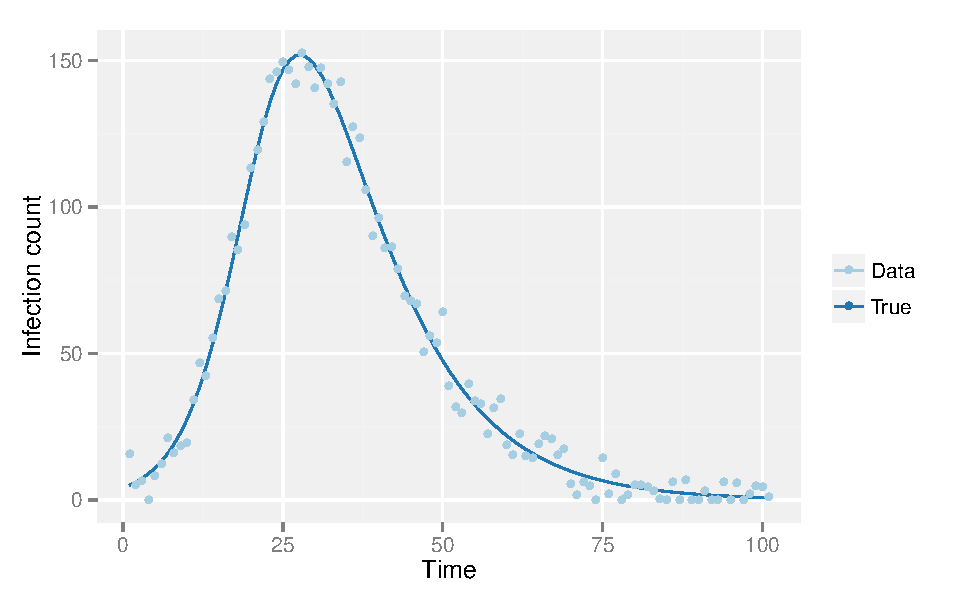
\includegraphics[width=\textwidth]{./images/dataplot.pdf}
        \caption{True SIR ODE solution infected counts, and with added observation noise. \label{mcmcdataplot}}
    \end{figure}

    The Hamiltonian MCMC model fitting was done using Stan (\url{http://mc-stan.org/}), a program written in \verb|C++| that does Baysian statistical inference using Hamiltonian MCMC. Stan's R interface (\url{http://mc-stan.org/interfaces/rstan.html}) was used to ease implementation.

    Throughout this paper, the explicit Euler integration scheme was used to obtain solutions to our ODE-based models. While this scheme is not the most accurate or efficient one available, it as chosen for its ease of implementation in the required languages and transparency with regards to stochastic processes, which have been added into later models. Using a more advanced integrator such as Runge-Kutta makes it harder to properly specify how stochastic process evolution should be handled, and would have required significantly more implementation work to boot. Hence, we have opted for the lo-fi solution we know will function the way we require.

    In order to use an Explicit Euler-like stepping method in the later Stan model, the synthetic observation counts were treated as weekly observations in which the counts on the other six days of the week were unobserved.

    Figure [\ref{traceplot}] shows the traceplot for the the post-burn-in chain data returned by the RStan fitting. We see that the chains are mixing well and convergence has likely been reached.

    \begin{figure}
        \centering
        \captionsetup{width=0.8\linewidth}
        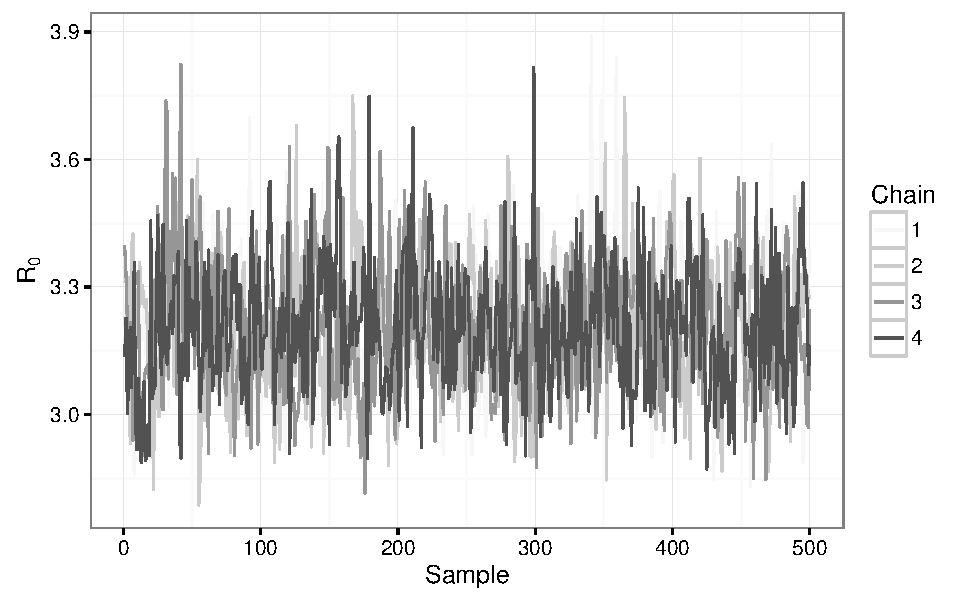
\includegraphics[width=\textwidth]{./images/traceplotR0.pdf}
        \caption{Traceplot of samples drawn for parameter $\mathcal{R}_0$, excluding burn-in. \label{traceplot}}
    \end{figure}

	Figure [\ref{traceplot2}] shows the chain data including the burn-in samples. We can see why it is wise to discard these samples (note the scale).

    \begin{figure}
        \centering
        \captionsetup{width=0.8\linewidth}
        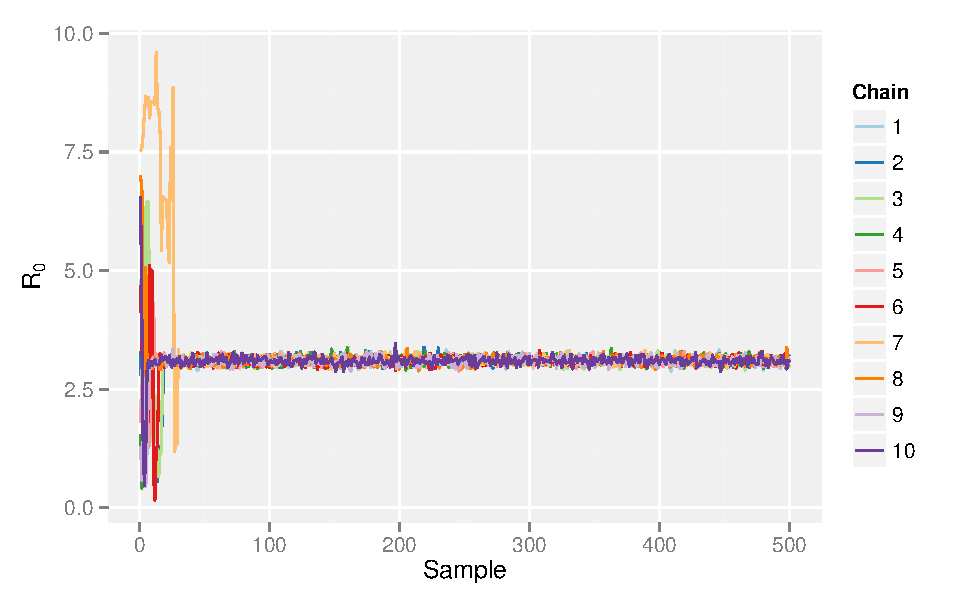
\includegraphics[width=\textwidth]{./images/traceplotR0_inc.pdf}
        \caption{Traceplot of samples drawn for parameter $\mathcal{R}_0$, including burn-in. \label{traceplot2}}
    \end{figure}

    Figure [\ref{hmckernels}] shows the the kernel density estimates for each of the model parameters and the initial number of cases. We see that while the estimates are not perfect, they are more than satisfactory.

    \begin{figure}
    	\centering
    	\captionsetup{width=0.8\linewidth}
        \begin{subfigure}[tl]{0.4\textwidth}
            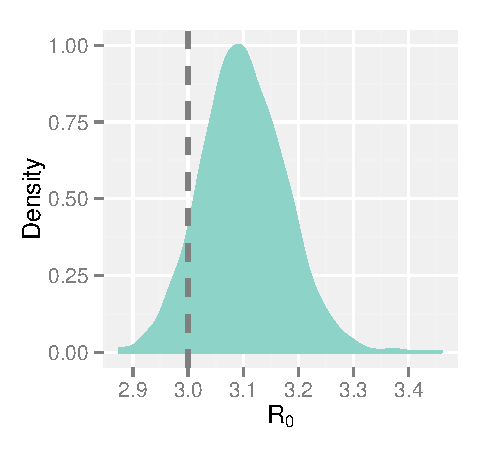
\includegraphics[width=\textwidth]{./images/kernelR0.pdf}
        \end{subfigure}
        \begin{subfigure}[tr]{0.4\textwidth}
            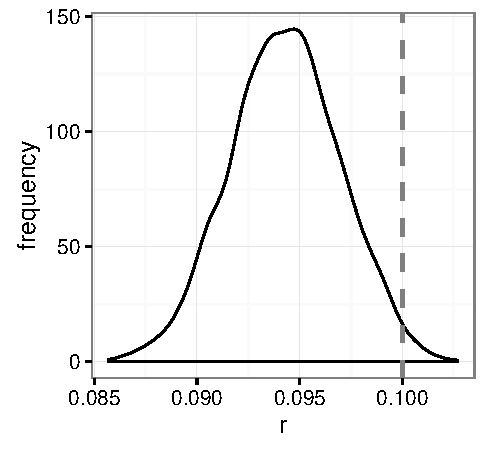
\includegraphics[width=\textwidth]{./images/kernelr.pdf}
        \end{subfigure}
        \begin{subfigure}[bl]{0.4\textwidth}
            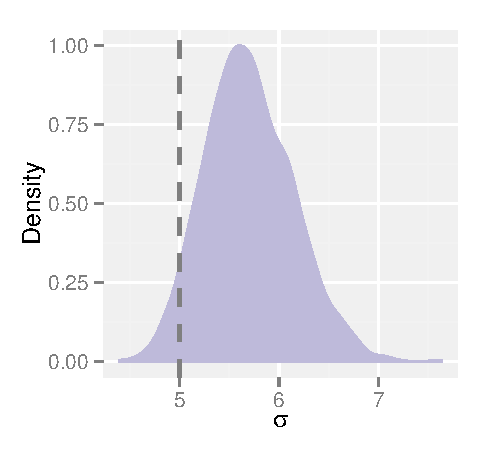
\includegraphics[width=\textwidth]{./images/kernelsigma.pdf}
        \end{subfigure}
        \begin{subfigure}[br]{0.4\textwidth}
            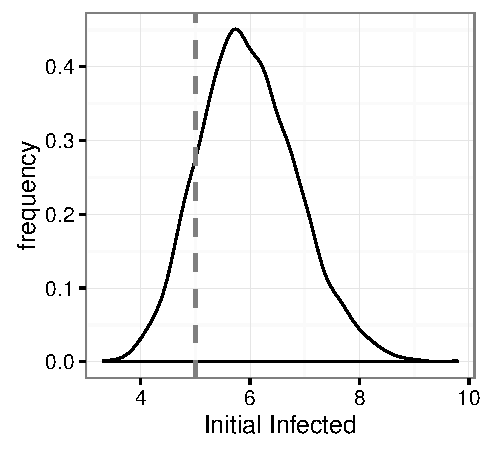
\includegraphics[width=\textwidth]{./images/kernelinfec.pdf}
        \end{subfigure}
        \caption{Kernel density estimates produced by Stan. Dashed lines show true parameter values. \label{hmckernels}}
    \end{figure}